\chapter{Background}

In this chapter we describe model architectures, concepts and training
methodologies our work uses.


\section{Text embedding}

To allow neural networks to process text, each continuous piece of text is
mapped to a series of vectors that represent it. This mapping and its result is
called an embedding. Traditionally we would split the input text
to sub-words and allow the network to change their embedding arbitrarily to
solve some end task. Example of such task is sub-word prediction, where the
network guesses masked-out sub-word.

In our work we train a network to map a long piece of text to a single vector.
As the size of the embedding is limited, we expect the network to effectively
compress the input. In this work our aim is not to reconstruct the input from
the embedding, but rather to capture both the structure and meaning of the text.

\section{Paragraph Vector}

Paragraph Vector~\cite{le2014distributed} (also known as Doc2Vec) is a
text-embedding model that is an extension of
Word2Vec~\cite{mikolov2013efficient}. Paragraph Vector is composed of two
sub-models called Distributed Memory (or DM) and Distributed Bag of Words (or
DBOW). Both DM and DBOW are trained on token prediction. To predict masked-out
tokens, both models use embedding of the whole input, while DM additionally
computes word embeddings. In practice, each embedded piece of text (a word or
an input) gets an identifier, which is used as an index into an embedding
matrix that stores the vector representations.

Paragraph Vector, thanks to its simplicity, can be trained quickly, even with
limited computational resources. Additionally the model can embed texts of any
length. However, Paragraph Vector has three major disadvantages. First, it
ignores text structure, by assuming the input is a bag of words rather than its
sequence. Second, because it is very simple model, it does not have the
capability to understand complex relationships of words, sentences or
paragraphs. Third, due to how embeddings are computed, the inference time is
very long, since it is necessary to train the model until convergence on the
previously unseen test input.

% TODO: my own graphic here

\begin{figure}[h]
    \centering
    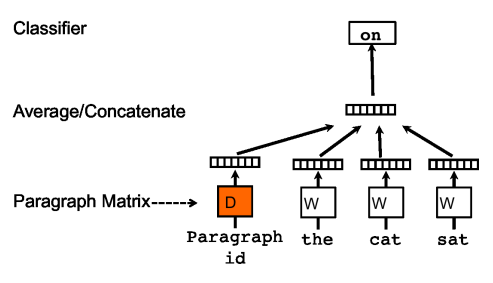
\includegraphics[width=0.4\textwidth]{./img/pv-dm.png}
    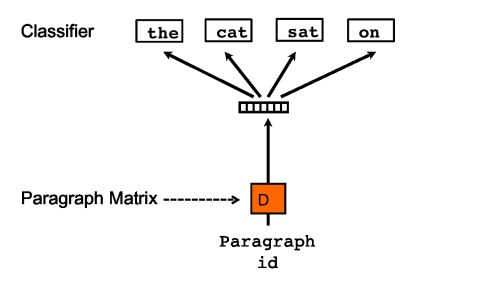
\includegraphics[width=0.4\textwidth]{./img/pv-dbow.png}
    \caption{PV-DM and PV-DBOW architectures.\label{fig:pv-dm_pv-dbow}}
\end{figure}

\section{SBERT}

Sentence-BERT~\cite{reimers2019sentence} (or SBERT) a composition of a
Transformer (TODO: citation) encoder with a pooling layer above its final
hidden states. The model is warm-started from a pre-trained Transformer such as
BERT (TODO: citation), RoBERTa (TODO: citation) or MPNet (TODO: citation). Then
it is fine-tuned on NLI datasets so that the pooled representations of the
whole inputs are comparable using cosine. The goal is that a semantic
difference between two inputs should correspond to the cosine between the
two pooled representations.

Thanks to higher parameter count, SBERT can understand more complex
relationships than Paragraph Vector. As no parameter adjustment is necessary
during inference, SBERT predicts embeddings very quickly which makes it
suitable for search applications. The disadvantage is that it can process text
only up to a certain length and unfortunately the same training cannot be used
for longer texts due to lack of appropriate datasets.

\section{Sparse attention}

Traditional Transformer encoder uses full-attention, which means that every
token can interact (or attend) to any other token. This type of attention
creates quadratic number of interactions to input length and therefore also
quadratic time and space complexity. This seriously limits use of transformers
for longer inputs even with efficient cuda kernels (TODO: really? Citation
needed). To overcome this issue, interactions between some tokens are ignored.
Such type of attention is called sparse.

TODO: My graphic of attentions

\begin{figure}[h]
    \centering
    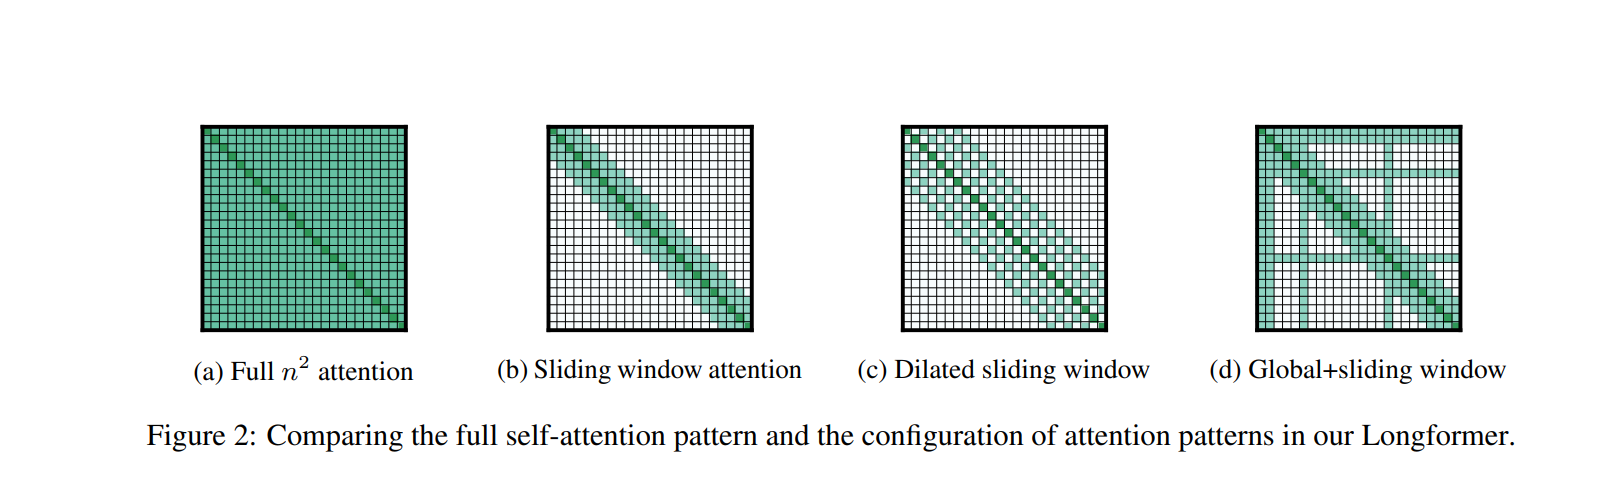
\includegraphics[width=0.9\textwidth]{./img/longformer_attention.png}
    \caption{Longformer attention matrix.\label{fig:longformer_sparse_att}}
\end{figure}

Sparse attention can have different designs but they are usually composed of
several types of mechanisms (such as sliding window, global, random -- I can
write more about this).

\subsection{Longformer}

Longformer~\cite{beltagy2020longformer}, is a transformer with sparse attention
that combines global and sliding window mechanisms. It is warm-started from
RoBERTa weights with its learned embeddings copied 4 times. Thus Longformer can
process inputs up to 4096 tokens long. Then the model was fine-tuned using
Masked Language Modelling (or MLM) on a dataset of long documents such as
Wikipedia articles or books.

There are many others sparse attention models, but we ephasize Longformer since
it is one of the best performing~\cite{tay2020long} and yet has relatively
simple attention mechanism, which makes it a suitable benchmark.

\section{Teacher-student training}

Teacher-student training is a setup in which we train a model (a student)
according to the relationship of its output with outputs of another model (a
teacher), which is frozen. The desired relationship can differ, but often we
aim to minimize the difference between the two outputs to simulate the teacher
model by the student. Teacher-student training can been used to dramatically
decrease the size of a model, while at the same time only slightly decreasing
its performance. Another use of this method is in multi-modal learning when
more modalities of the same input are available. In such cases we can have
several teacher models, each for different modality, providing their outputs to
the loss of a single student model.

TODO: some graphic

\section{Canonical Correlation Analysis}

Canonical Correlation Analysis (CCA) computes linear projections of two vectors
such that their projections are maximally correlated. To define CCA properly,
let us look at its mathematical formulation.

\begin{defn}[Canonical Correlation Analysis]\label{def:cca}

  For two matrices $X_1 \in \mathbb{R}^{n_1 \times m_1}$ and $X_2 \in
  \mathbb{R}^{n_2 \times m_1}$, Canonical Correlation Analysis finds $p \in
  \mathbb{R}^m_1$ and $q \in \mathbb{R}^m_2$ that maximize

  \begin{equation}
    \begin{split}
      & corr(X_1p, X_2q) = \frac{p^TX_1^TX_2q}{||Xp|| ||Yq||} \\
      \text{s.t.}\quad &||X_1p|| = ||X_2q|| = 1 \\
    \end{split}
  \end{equation}


\end{defn}

Definition~\ref{def:cca} suggests that CCA gives only a single number as the
measure of correlation of two matrices. When the dimensions of the input
vectors are large enough, however, often there is a some combination of
features that results in correlation of 1. This would make CCA relatively
useless in context of high-dimensional spaces. To overcome this issue we assume
multiple correlations for several mutually orthogonal projections. Again, let
us look at the mathematical formulation.

\begin{defn}[Canonical Correlation Analysis in more dimensions]\label{def:cca_more_dim}

  For two matrices $X_1 \in \mathbb{R}^{n_1 \times m_1}$ and $X_2 \in
  \mathbb{R}^{n_2 \times m_1}$, Canonical Correlation Analysis in $k$
  dimensions finds $P \in \mathbb{R}^{m_1 \times k}$ and $Q \in \mathbb{R}^{m_2
  \times k}$ that maximize

  \begin{equation}
    \begin{split}
      &\sum_{i = 1}^k corr(X_1P_{*i}, X_2Q_{*i}) \\
      \text{s.t.}\quad &P^TX_1^TX_1P = I_k = Q^TX_2^TX_2Q \\
    \end{split}
  \end{equation}


\end{defn}

If we consider the conditions in Definition~\ref{def:cca_more_dim}, the
resulting value can be easily formulated as $trace(P^TX_1^TX_2Q) =
trace(P^T\Sigma_{X_1X_2}Q)$, where $\Sigma_{X_1X_2}$ is covariance matrix of
$X_1$ and $X_2$.

TODO: analytical solution to pure CCA

\subsection{CCA as a loss}

CCA can be used as a loss in teacher-student training to establish some sort of
correspondence between the teacher's and the student's outputs. When CCA is
maximized the teacher's and the student's outputs are first linearly
transformed, before the correlation is computed. CCA is therefore weaker
requirement than classical correlation.

The problem of using CCA as a loss is that it is defined in the context of the
whole dataset rather than just a minibatch. It is therefore unclear how CCA for
a pair of minibatches of vectors should be computed. Someone (TODO: citation)
found that using large enough batch size is sufficient for the training to
converge.

\subsection{Deep CCA}

Deep CCA (or DCCA) is an extension of CCA that computes projections using
neural networks. As such it is more powerful than plain CCA as it allows for
non-linear projections. To compute DCCA the network has to be trained on the
pairs of vectors with CCA as its loss.

TODO: graphic of architecture

If CCA is weaker condition than just correlation, DCCA is even weaker since
there is no limit to how the projections should look like.

\subsection{Soft CCA}

Soft CCA reformulates CCA and thus allows its straightforward use in the
context of minibatches. With constraints from Definition~\ref{def:cca_more_dim}
taken into account, CCA can be formulated using Forbenious matrix norm:

\begin{align}
  P^\ast, Q^\ast &= \underset{P, Q}{\argmin} ||X_1P - X_2Q||^2_F \\
  &= \underset{P, Q}{\argmin} trace\Big((X_1P - X_2Q)^T(X_1P - X_2Q)\Big) \\
  &= \underset{P, Q}{\argmin} {-2} trace(P^TX_1^TX_2Q) \\
  &= \underset{P, Q}{\argmax} trace(P^TX_1^TX_2Q) \\
  &= \underset{P, Q}{\argmax} \sum_{i = 1}^k corr(X_1P_{*i}, X_2Q_{*i})
\end{align}

So, in essence minimizing CCA is the same as minimizing the difference between
projections, whose features are decorrelated. This is the formulation Soft CCA
builds on. Soft CCA decomposes CCA into to parts:

\begin{itemize}
  \item minimization of the difference between projections

    \begin{equation}
      ||X_1P - X_2Q||^2_F
    \end{equation}

  \item decorrelation of each projection $P$

    \begin{equation}
      \sum_{i \ne j} (P^TX^T_{mini}X_{mini}P)_{ij} = \sum_{i \ne j} \Sigma_{X_{mini}P},
    \end{equation}

    where $X_{mini}$ is batch-normalized minibatch.

\end{itemize}

To bring correlation matrix of the current minibatch $\Sigma_{X_{mini}P}$
closer to the true covariance, the decorrelation part is in fact computed from
a covariance matrix that is increamentally learned.

In this way Soft CCA increamentally decreases CCA through incrementally learned
approximation of the projections' covariances.

\section{Contrastive loss}

Contrastive losses are types of losses which compare several model's outputs to
each other and based on this comparison they compute a value, which can be used
as a loss. Contrastive loss is often used when the model's goal is to
understand and distinguish different inputs. In this setting, we would penalize
the model if the representations of similar inputs are far apart or if the
representations of different inputs are close. Similar inputs are called
positives, whereas distinct inputs are called negatives.

When no supervised information about the similarity of a pair of inputs is
available, we can use in-batch outputs as negatives. Here we automatically
assume that all our inputs are distinct and that the model should distinguish
between all of them.
